\documentclass[10pt, landscape, a4paper]{article}
\usepackage{geometry}[landscape]
\usepackage{multicol}
\usepackage{graphicx}
\usepackage{amsmath} 
\usepackage{amssymb}
\usepackage{ccicons}
\usepackage{hyperref}

\usepackage[dvipsnames]{xcolor}

% Set page margins
\geometry{top=.8cm, left=.8cm, right=.8cm, bottom=.8cm}

% Set paragraph indentation
\setlength{\parindent}{0pt}

% Set path for assets
\graphicspath{{assets/}}

\setlength{\columnsep}{20pt}
\raggedcolumns

% _____ CUSTOM COMMANDS __________________________________________
\newcommand{\E}[0]{\mathbb{E}}
\newcommand{\R}[0]{\mathbb{R}}

\newcommand{\sgn}[0]{\text{sgn}}

\newcommand{\argmin}[1]{\underset{#1}{\text{argmin}}}
\newcommand{\argmax}[1]{\underset{#1}{\text{argmax}}}

\begin{document}
\begin{multicols*}{3}

% _____ CONTENT __________________________________________________

% main heading
\begin{center}
	\Large{\textbf{Computer Systems}} \\
    \small{by dcamenisch}
\end{center}

\section{Introduction}

This document is a summary of the 2022 edition of the lecture \textit{Computer Systems} at ETH Zurich. I do not guarantee correctness or completeness, nor is this document endorsed by the lecturers. If you spot any mistakes or find other improvements, feel free to open a pull request at \url{https://github.com/DannyCamenisch/systems-summary}. This work is published as CC BY-NC-SA.

\begin{center}
	\ccbyncsa
\end{center}
\section{Naming}

Naming is a fundamental concept, it allows resources to be bound at different times. Names are bound to objects, this is always relative to a context. One example of this would be path names, e.g. \textit{/usr/bin/emacs}. Name resolution can be seen as a function from context and name to some object. The resolved object can be a context in itself. This gives us a naming network.
\begin{center}
	\includegraphics[width=0.8\linewidth]{naming-network.png}
\end{center}

Both synonyms (two names bound to the same object) and homonyms (the same name bound to two different objects) can occur.
\section{The Kernel}

There are three main functions to an OS. Commonly they are referred to from a designer's view, but the user's view can be much more helpful to actually understand how it works.

\begin{center}
	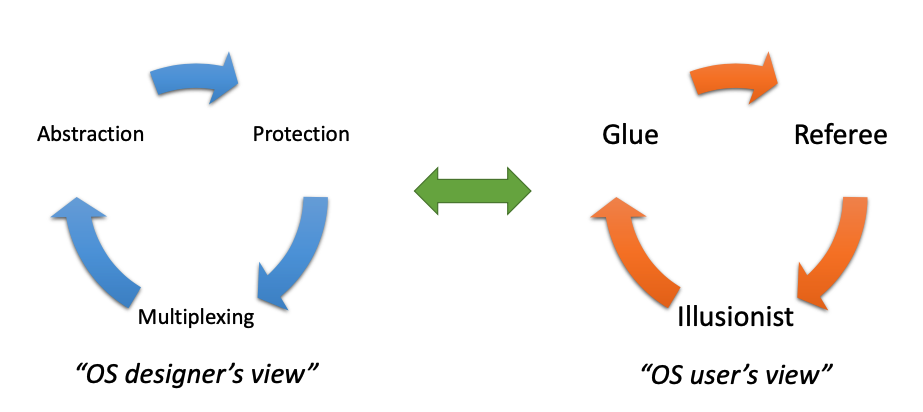
\includegraphics[width=\linewidth]{os-functions.png}
\end{center}


\subsection{Bootstrapping}

The term bootstrapping refers to pulling himself up from his own boots. In computer systems it is what we call the process of starting up a computer (booting). This boot process looks like this:

\begin{enumerate}
	\item CPU starts executing code at a fixed address (Boot ROM)
	\item Boot ROM code loads 2nd stage boot loader into RAM
	\item Boot loader loads kernel and optionally initials file system into RAM
	\item Jumps to kernel entry point
\end{enumerate}

The first few lines are always written in assembly, but generally we want to switch to C as soon as possible.


\subsection{Mode Switch}

One of our main goals is to protect the OS from applications that could harm it (intentionally or not). For this purpose we introduce two different modes:

\begin{itemize}
	\item \textbf{Kernel Mode} - execution with full privileges, read/write to any memory, access and I/O, etc. Code here must be carefully written
	\item \textbf{User Mode} - limited privileges, only those granted by the OS kernel
\end{itemize}

These two (or more) modes are already implemented in hardware. The main reason for a mode switch is when we encounter a processor exception (mode switch from user to kernel mode). If this is the case, we want the following to happen:

\begin{enumerate}
	\item Finish executing current instruction
	\item Switch mode from user to kernel
	\item Look up exception cause in exception vector table
	\item Jump to this address
\end{enumerate}

Further we may also want to save the registers and switch page tables. When switching between the modes we also have to change our address space, but we might want to access some informations from the user mode address space. One way of doing this is to use a so called \textbf{trampoline}, which is a part of the address space that gets mapped to the same location in user and kernel mode.

\begin{center}
	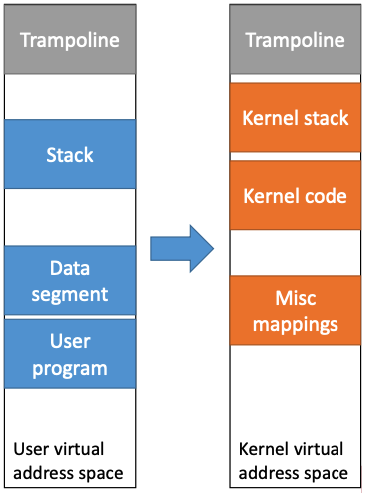
\includegraphics[width=0.4\linewidth]{trampoline.png}
\end{center}

Mode switches can also occur the other way around (from kernel mode to user mode). The main reasons for this are:

\begin{itemize}
	\item New process / thread start
	\item Return from exception
	\item Process / thread context switch
	\item User-level upcall (UNIX signal)
\end{itemize}

This leads us to the following perspective:

\begin{center}
	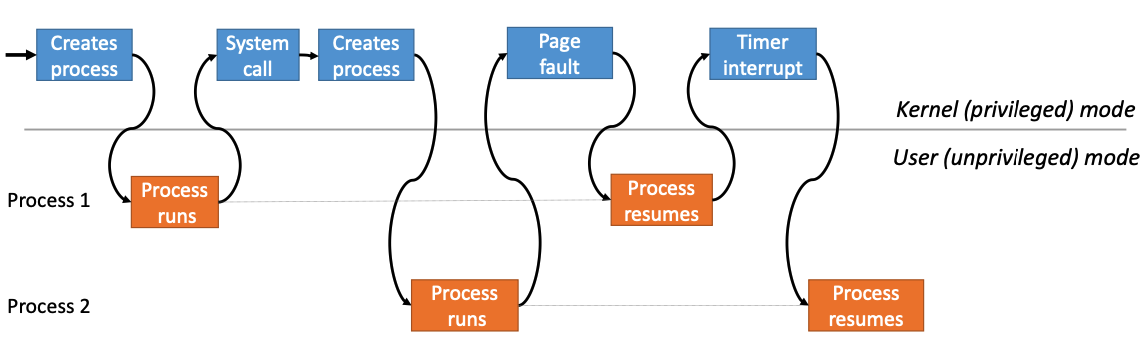
\includegraphics[width=\linewidth]{mode-switch.png}
\end{center}

The mode switch is fundamental to modern computers:

\begin{itemize}
	\item It enables virtualization of the processor
	\item It creates the illusion of multiple computers
	\item It referees access to the CPU
\end{itemize}


\subsection{General Model of OS Structure}

\begin{center}
	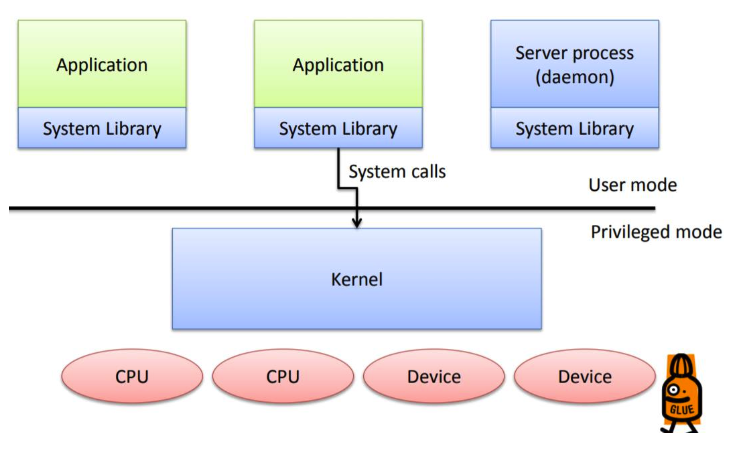
\includegraphics[width=0.9\linewidth]{os-structure.png}
\end{center}

\begin{itemize}
	\item \textbf{Kernel}: The kernel consists of software run in privileged mode. There might be more than one kernel in an OS. It can handle system calls, h/w interrupts etc.
	\item \textbf{System Libraries}: They are part of any application run on the machine and should provide an interface for the kernel.
	\item \textbf{Daemon}: This is a process running as part of the OS. It’s not run in privileged mode and may use system libraries. An example might be a file system.
\end{itemize}

We can differentiate between monolithic kernels and microkernels, depending on the amount of code in kernel mode.


\subsection{System Calls}

System calls are the only way for user mode programs to enter kernel mode. System calls are a type of exception, but they try to look a lot more like a procedure call. Therefore the kernel system call handler has to first locate arguments, copy these arguments into kernel memory, validate these arguments and then copy the results back into user memory after execution. An example of such a system call would be \textit{write()}. 


\subsection{Hardware Timers}

What happens if a user mode program does not cause any exception and does not give control back to the kernel? Hardware timers are a solution for this problem, the hardware device periodically interrupts the processor and returns control to the kernel handler, which sets the time of the next interrupt.

\section{Processes}

When you run a program, the OS creates a process to execute the program in. A process is an illusion created by the OS, it creates an execution environment for a program. This environment gives the program limited rights (access, name spaces, threads, etc.) and therefore it is both a security and a resource principal.


\subsection{Creating a Process}

There are two main approaches to creating new processes:

\begin{itemize}
	\item \textbf{Spawn} - constructs a running process from scratch
	\item \textbf{Fork / Exec} - creates a copy of the calling process or replaces the current program with another in the same process
\end{itemize}

\textbf{Spawn}

\begin{itemize}
	\item Create and initialize the process control block (PCB) in the kernel
	\item Create and initialize a new address space
	\item Load the program into the address space
	\item Copy arguments into memory in the address space
	\item Initialize the hardware context to start execution at "start"
	\item Inform the scheduler that the new process is ready to run
\end{itemize}

Spawn is very complex, we have to specify everything about the new environment. If we omit a key argument a new process might have insufficient rights or resources or it might fail to function due to a security fault. \medskip

\textbf{Fork}

Fork on the other hand is less complex. The child process is almost an exact copy of the parent, with a different PID. We know which process we are in from the return value of the \textit{fork()} call ($0$ for child, $>0$ for parent, $<0$ for error). The complete UNIX process management API also includes:

\begin{itemize}
	\item \textit{exec()} - system call to change the program being run by the current process
	\item \textit{wait()} - system call to wait for a process to finish
	\item \textit{signal()} - system call to send a notification to another process
\end{itemize}

In contrast to \textit{spawn()}, here the child revokes rights and access explicitly before \textit{exec()}, further we can use the full kernel API to customize the execution environment.


\subsection{The Process Control Block}

The PCB is the main kernel data structure used to represent a process. It has to hold or refer to the page table, trap frame, kernel stack, open files, program name, scheduling state, PID, etc.


\subsection{Process Context Switching}

Context switching is the process of switching between different processes running in user mode or kernel mode. It is one of the key elements of the illusion that multiple programs can run in parallel. \columnbreak

There are two main reasons for the kernel to switch processes: either when a process has run for too long and gets interrupted by a hardware timer or when a process blocks. The second case happens when a system call can not complete immediately. The process then often calls \textit{sleep()} and other processes can be executed.
\begin{center}
	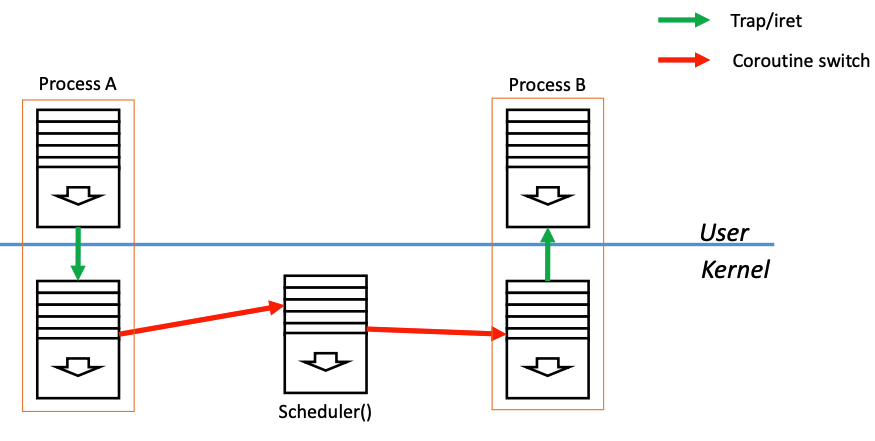
\includegraphics[width=\linewidth]{context-switching.png}
\end{center}


\subsection{Process Hierarchy}

By forking and spawning new processes we create sort of a hierarchy. If a child process dies, but the parent does not call \textit{wait()}, the child process becomes a zombie - it is dead, but still around since nobody asked for the return code. If a parent dies, but the child does not, the child becomes an orphan and gets reparented to the first process (PID \#1, \textit{init}).
\begin{center}
	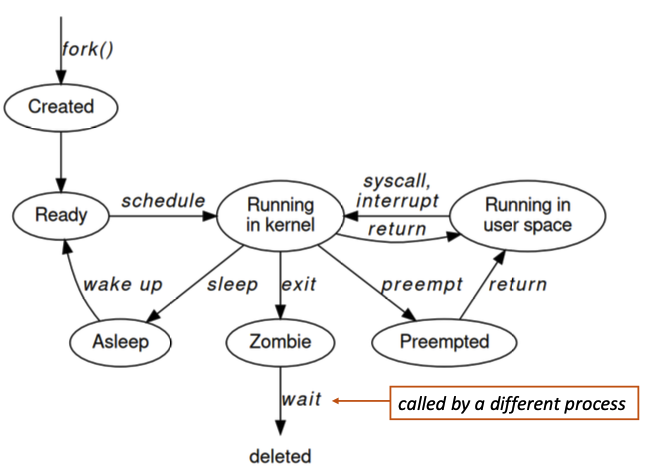
\includegraphics[width=\linewidth]{process-life-cycle.png}
\end{center}

The \textit{init} process is basically an infinite loop calling \textit{wait}(NULL), it gets rid of any zombies.


\subsection{Threads}

Threads are used as an abstraction for concurrency. They allow the usage of parallel hardware, e.g. multiple cores. A thread basically consist of a stack and some register values.\medskip

There is a distinction between \textbf{user threads} and \textbf{kernel threads}. The former are implemented entirely in user’s process. If a user thread is about to block (e.g. when executing a system call), the thread library usually interrupts this call and does something non blocking instead while the system call is served. Kernel threads are implemented by the OS kernel directly. They thus appear as different virtual processors to the user process. In this model, a set of threads share a virtual address space together. Each thread is now scheduled by the kernel itself, which keeps track of threads are part of which process. However, this makes the kernel more complicated.


\end{multicols*}
\end{document}

% ____ FOOTER ______________________________________________________
% Content and Template: 
% original by Danny Camenisch (dcamenisch@inf.ethz.ch), 2022
% based on different summaries from many helpful people